\section{Problem 5: Drude Model}

\subsection{Results}

\subsubsection{Current Density vs. Electric Field Strength}
%
The relationship between absolute current density and electric field strength is shown in Fig. (\ref{absolute_current_density}). This relationship is linear.
\begin{figure}[h]
    \centering
    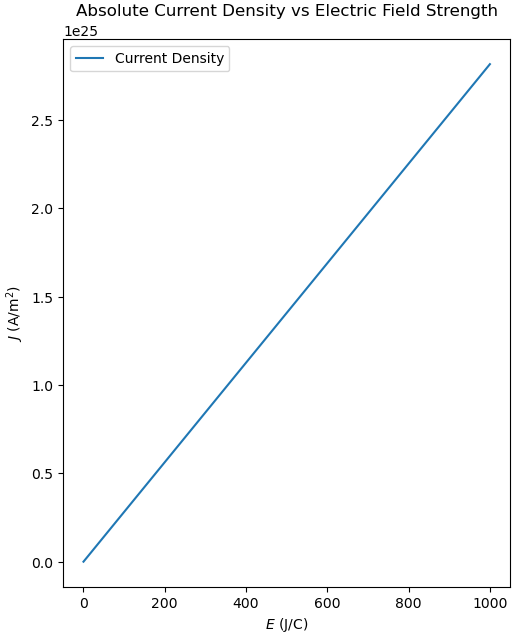
\includegraphics[width=10cm]{absolute_current_density.png}
    \caption{Absolute Current Density vs Electric Field Strength}
    \label{absolute_current_density}
\end{figure}
\begin{table}[h]
\begin{center}
    \begin{tabular}{|c|c|c|}
        \hline
        \textbf{System Parameter} & \textbf{Value} & \textbf{Notes} \\ \hline
        Carrier Density & 1$\times 10^{30}$ kg & arbitrary \\ \hline
        Carrier Charge & 1.602$\times 10^{-19}$ kg & Charge of One (1) Electron \\ \hline
        Effective Mass & 9.109$\times 10^{-31}$ kg & Mass of One (1) Electron \\ \hline
        Relaxation Time & 1 s & arbitrary \\ \hline
    \end{tabular}
\end{center}
\caption{System Parameters for Fig. (\ref{absolute_current_density})}
\label{system_parameters_for_absolute_current_density}
\end{table}

\subsubsection{Resistivity vs. Relaxation Time}
The relationship between resistivity and relaxation time is shown in Fig. (\ref{resistivity}). They are inversely proportional to each other.
\begin{figure}[h]
    \centering
    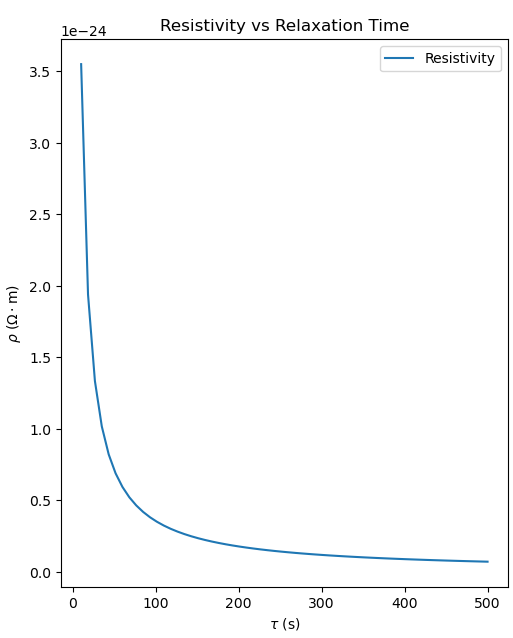
\includegraphics[width=10cm]{resistivity.png}
    \caption{Resistivity vs Relaxation Time}
    \label{resistivity}
\end{figure}
\begin{table}[h]
\begin{center}
    \begin{tabular}{|c|c|c|}
        \hline
        \textbf{System Parameter} & \textbf{Value} & \textbf{Notes} \\ \hline
        Carrier Density & 1$\times 10^{30}$ kg & arbitrary \\ \hline
        Carrier Charge & 1.602$\times 10^{-19}$ kg & Charge of One (1) Electron \\ \hline
        Effective Mass & 9.109$\times 10^{-31}$ kg & Mass of One (1) Electron \\ \hline
    \end{tabular}
\end{center}
\caption{System Parameters for Fig. (\ref{resistivity})}
\label{system_parameters_for_resistivity}
\end{table}


\subsection{Discussion}

A drift velocity $\mathbf{v}_d$ for charge carriers in the Drude model of a metal can be defined since the charge carriers are prohibited from accelerating indefinitely by collisions with the metal host atoms.